\section{N-grams language models}\label{sec:n-grams}

An n-gram is a contiguous sequence of items (typically letters or words) that are extracted from an information source (normally text, speech, images or \gls{dna}). By counting the n-grams in a knowledge corpus they can be used to create probabilistic language models for predicting the next item given a context. This is useful when developing speech recognizers and \gls{ocr} systems because the n-gram language model can help disambiguate items in the recognition process. Moreover they can be used for implementing text generators or suggestion / auto-complete systems and can also be applied to improve the efficiency of compression / search algorithms.



\subsection{Rank-frequency graphs}

Rank-frequency graphs are useful to analyze the word / n-gram diversity of a given text corpus. They are usually plotted in logarithmic scale and have the word rank in the X axis and the word frequency in the Y axis. They are also useful to check if a given text corpus follows the Zipf's law \cite{Piantadosi2014}, which states that the frequency of a given word in a text corpus is inversely proportional to its rank in the frequency table (as shown in \cref{eq:zipf-law}).

\begin{equation}\label{eq:zipf-law}
f(r) \propto \frac{1}{r^\alpha}
\end{equation}

Analyzing \crefrange{fig:rank-frequency-unigram}{fig:rank-frequency-pentagram} it can be seen that the dataset unigrams to pentagrams follow roughly the Zipf's law. Moreover, the alpha value introduced in \cref{eq:zipf-law} that best fits the plotted data starts at 0.25 in the first plot section, then increases to 0.5 in the middle plot section and becomes 1.0 in the last plot section. This is a typical behavior found in most languages \cite{NemethZainko2003}.

\begin{figure}[hb]
	\centering
	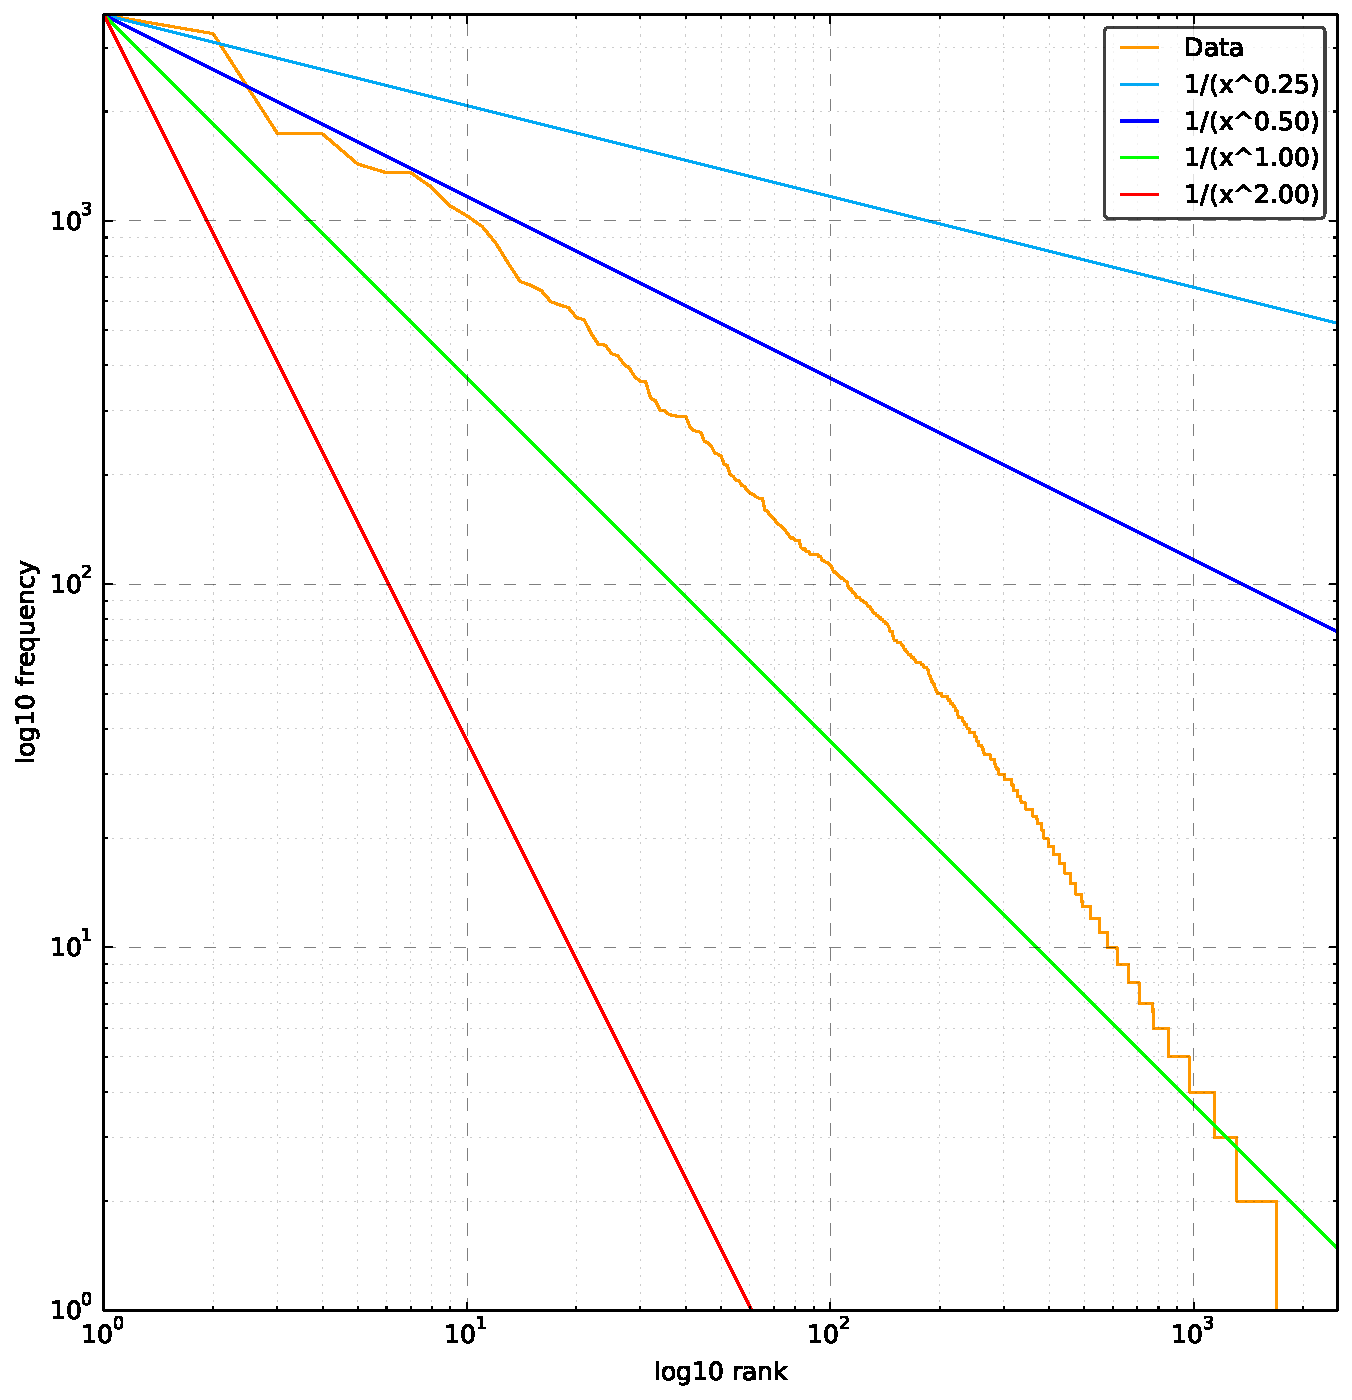
\includegraphics[width=0.9\linewidth]{figures/frequency-graphs/1-gram}
	\caption{Unigram rank-frequency graph of tokenized dataset}
	\label{fig:rank-frequency-unigram}
\end{figure}

\begin{figure}[ht]
	\centering
	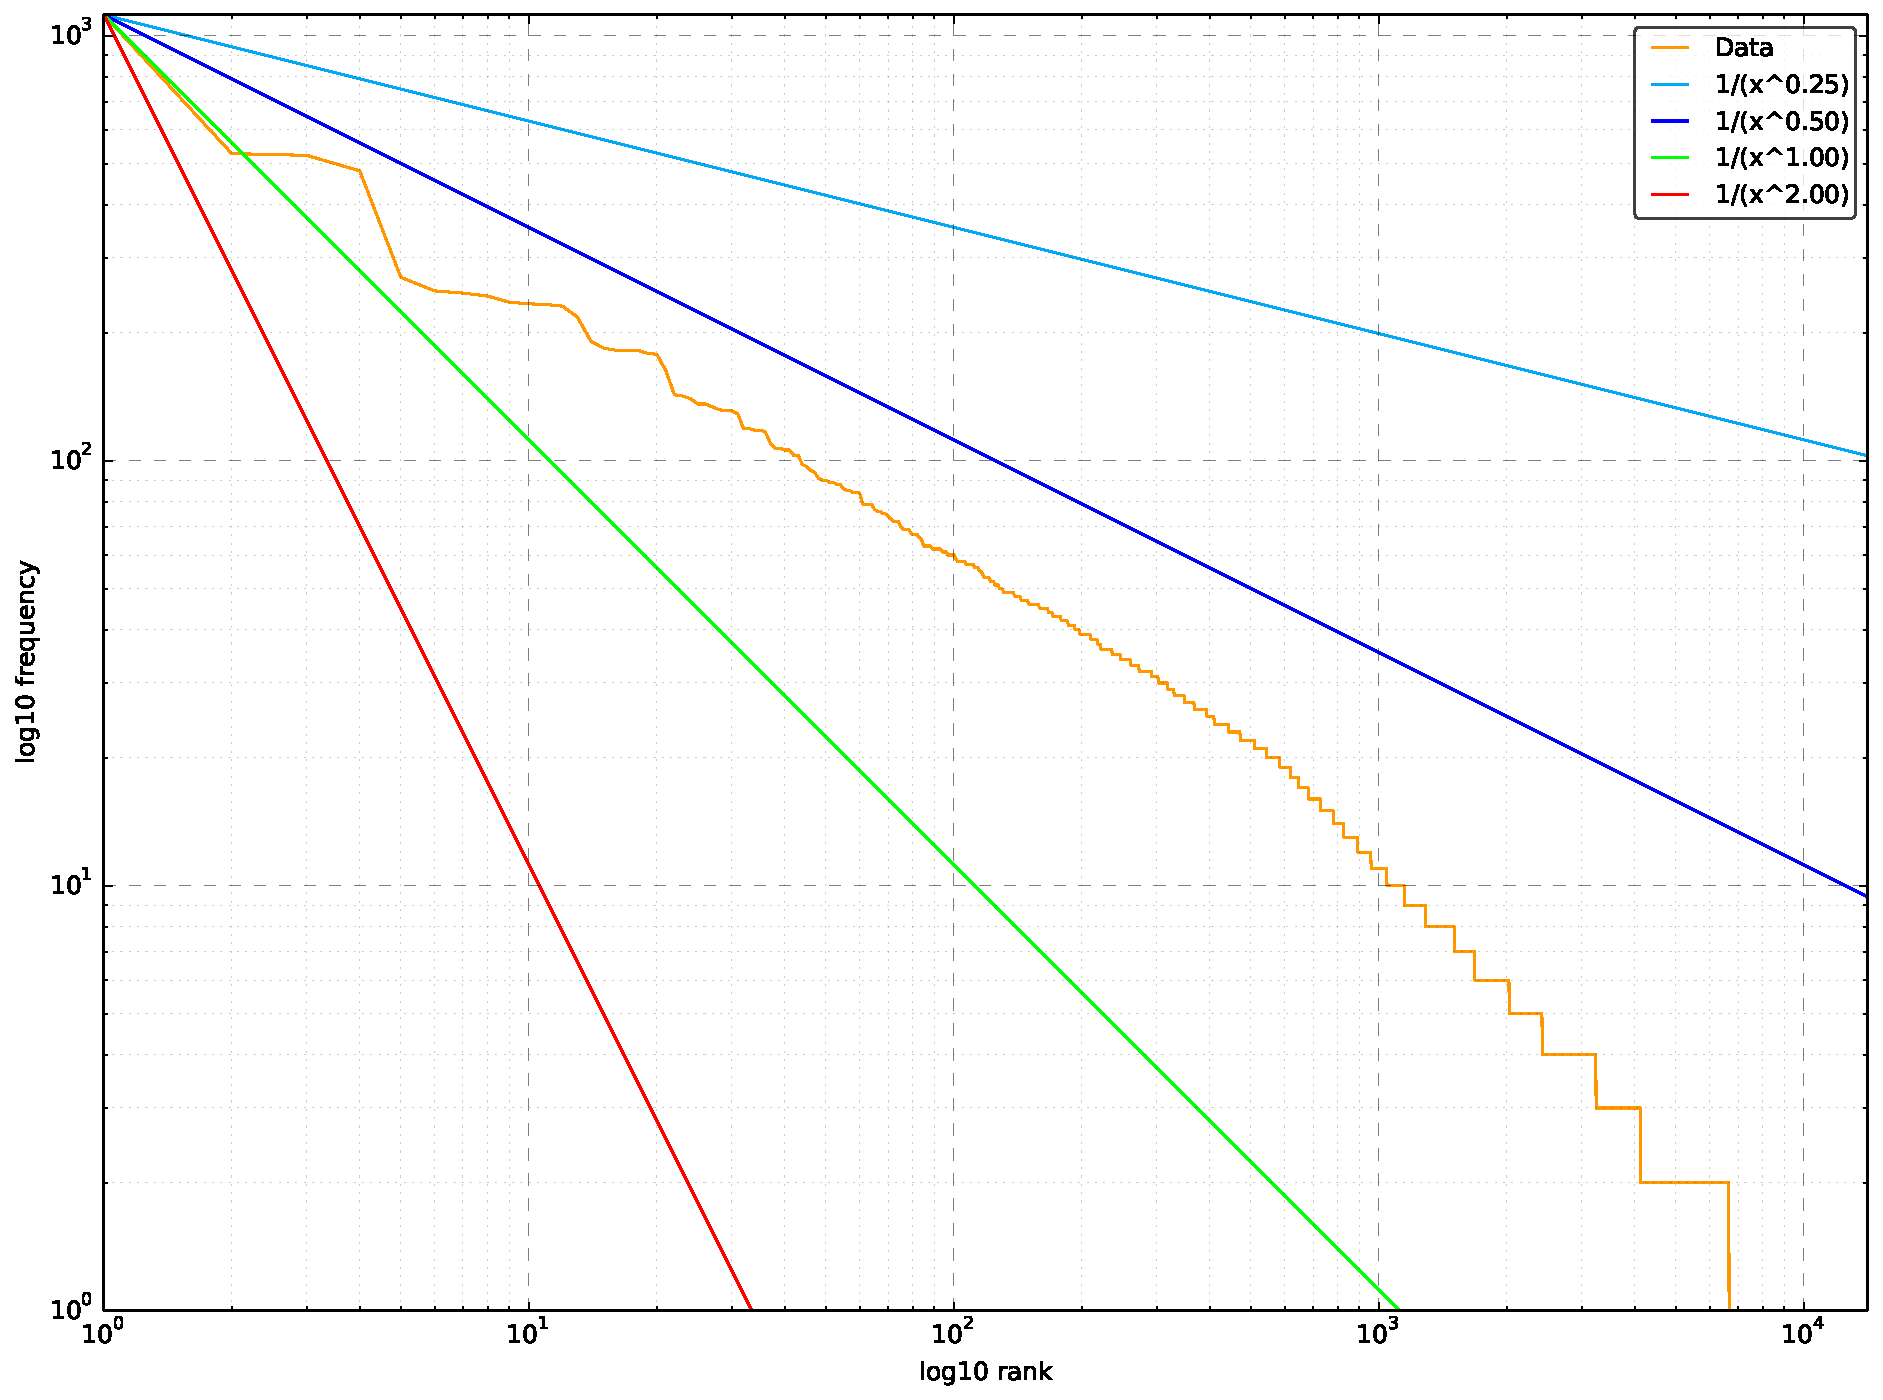
\includegraphics[width=0.9\linewidth]{figures/frequency-graphs/2-gram}
	\caption{Bigram rank-frequency graph of tokenized dataset}
	\label{fig:rank-frequency-bigram}
\end{figure}

\begin{figure}[ht]
	\centering
	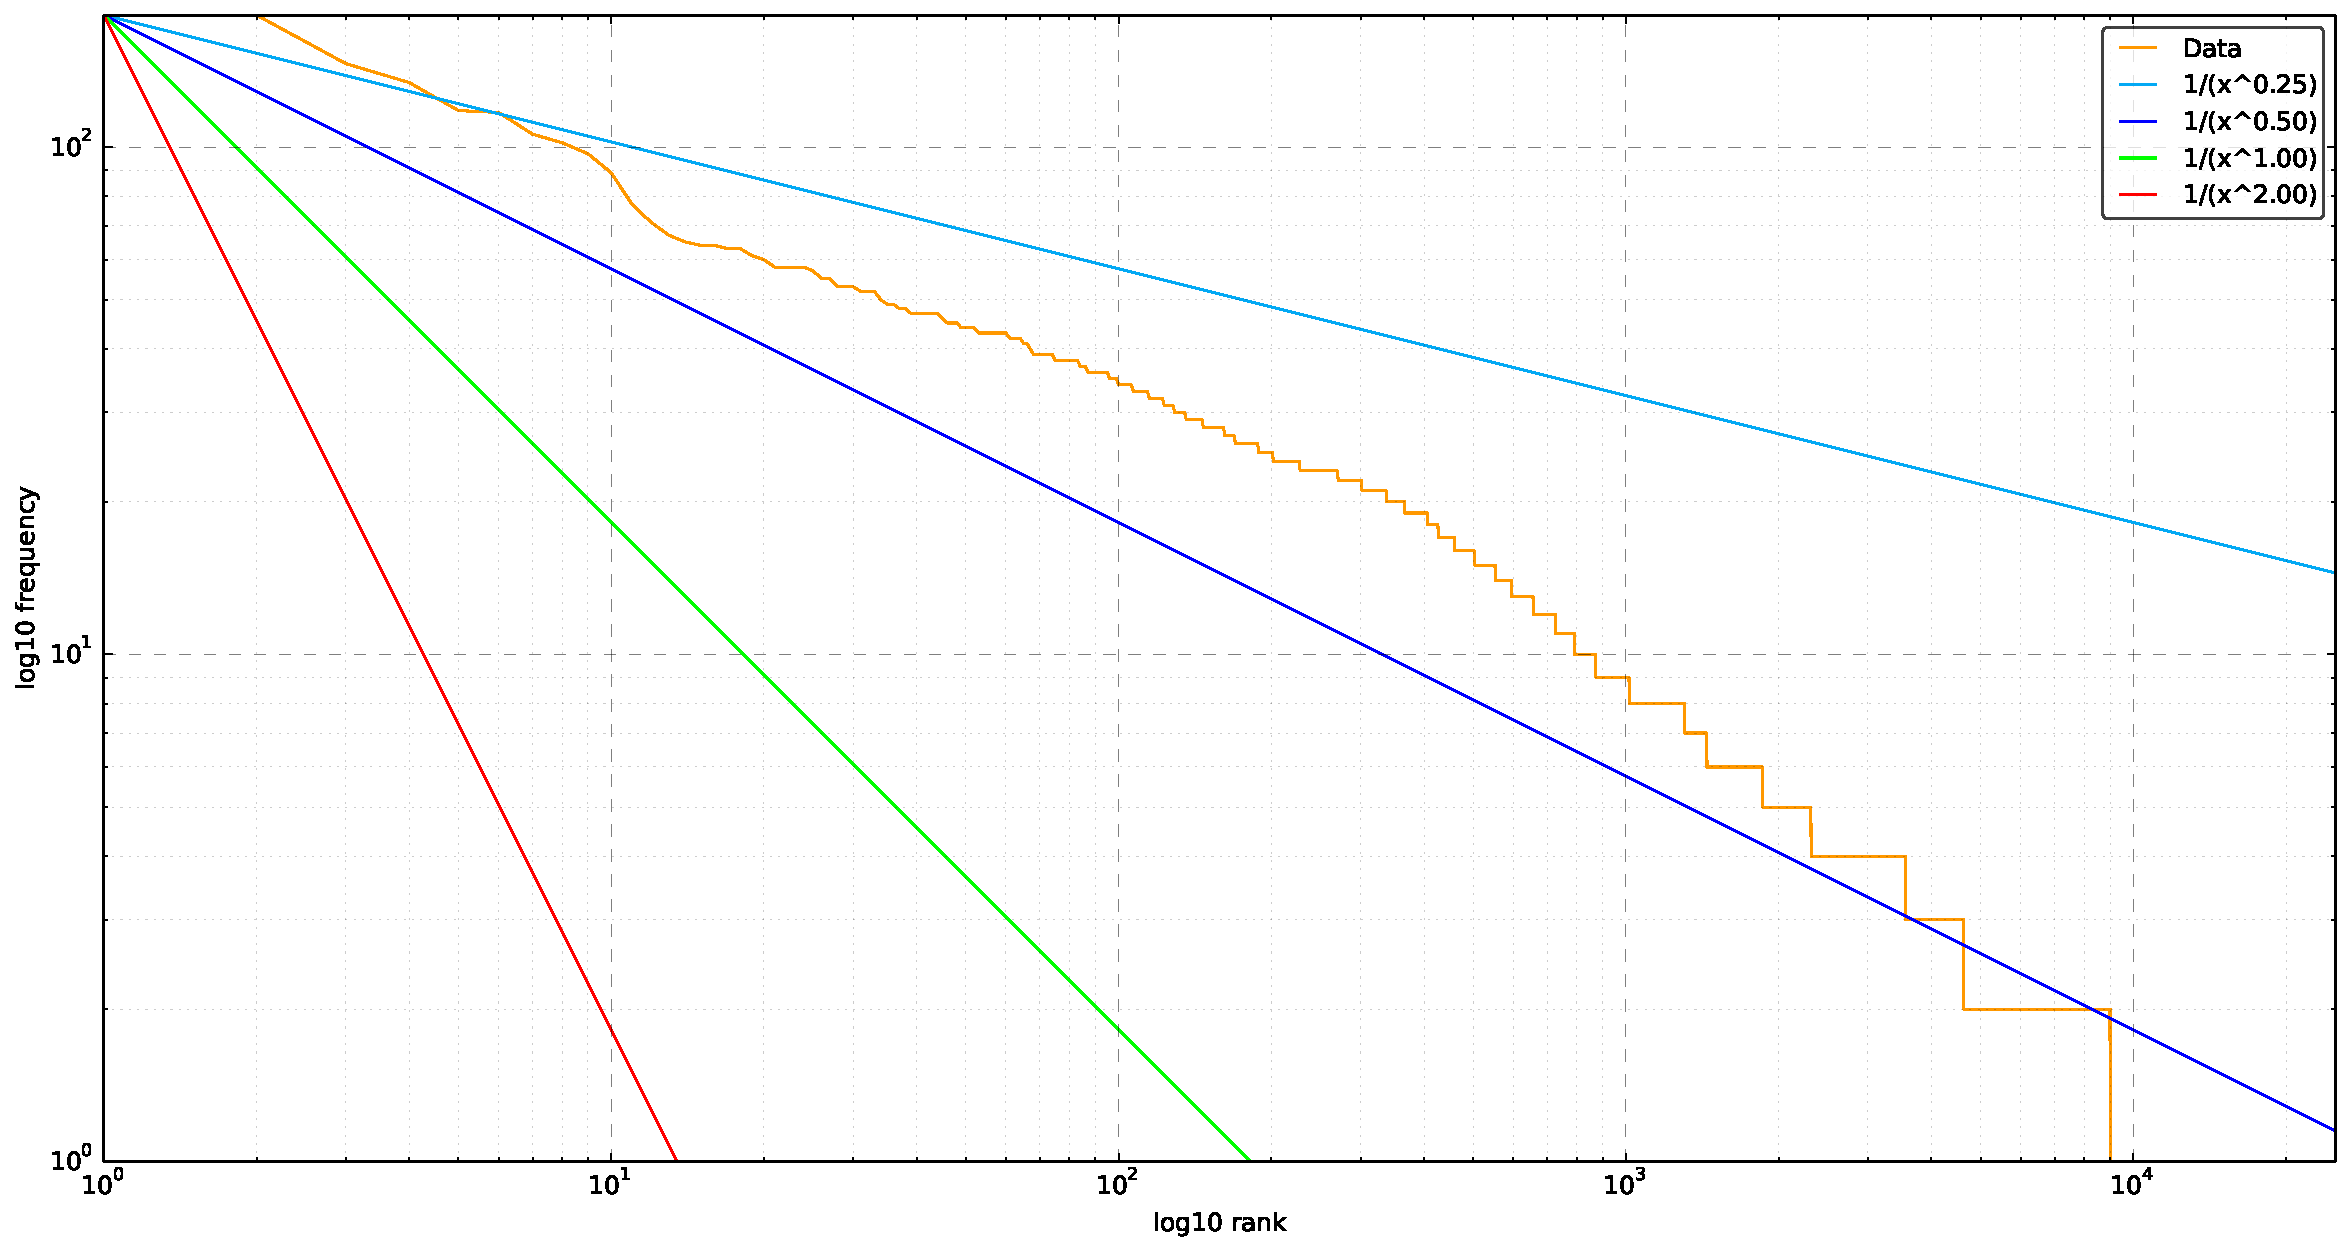
\includegraphics[width=0.9\linewidth]{figures/frequency-graphs/3-gram}
	\caption{Trigram rank-frequency graph of tokenized dataset}
	\label{fig:rank-frequency-trigram}
\end{figure}

\begin{figure}[ht]
	\centering
	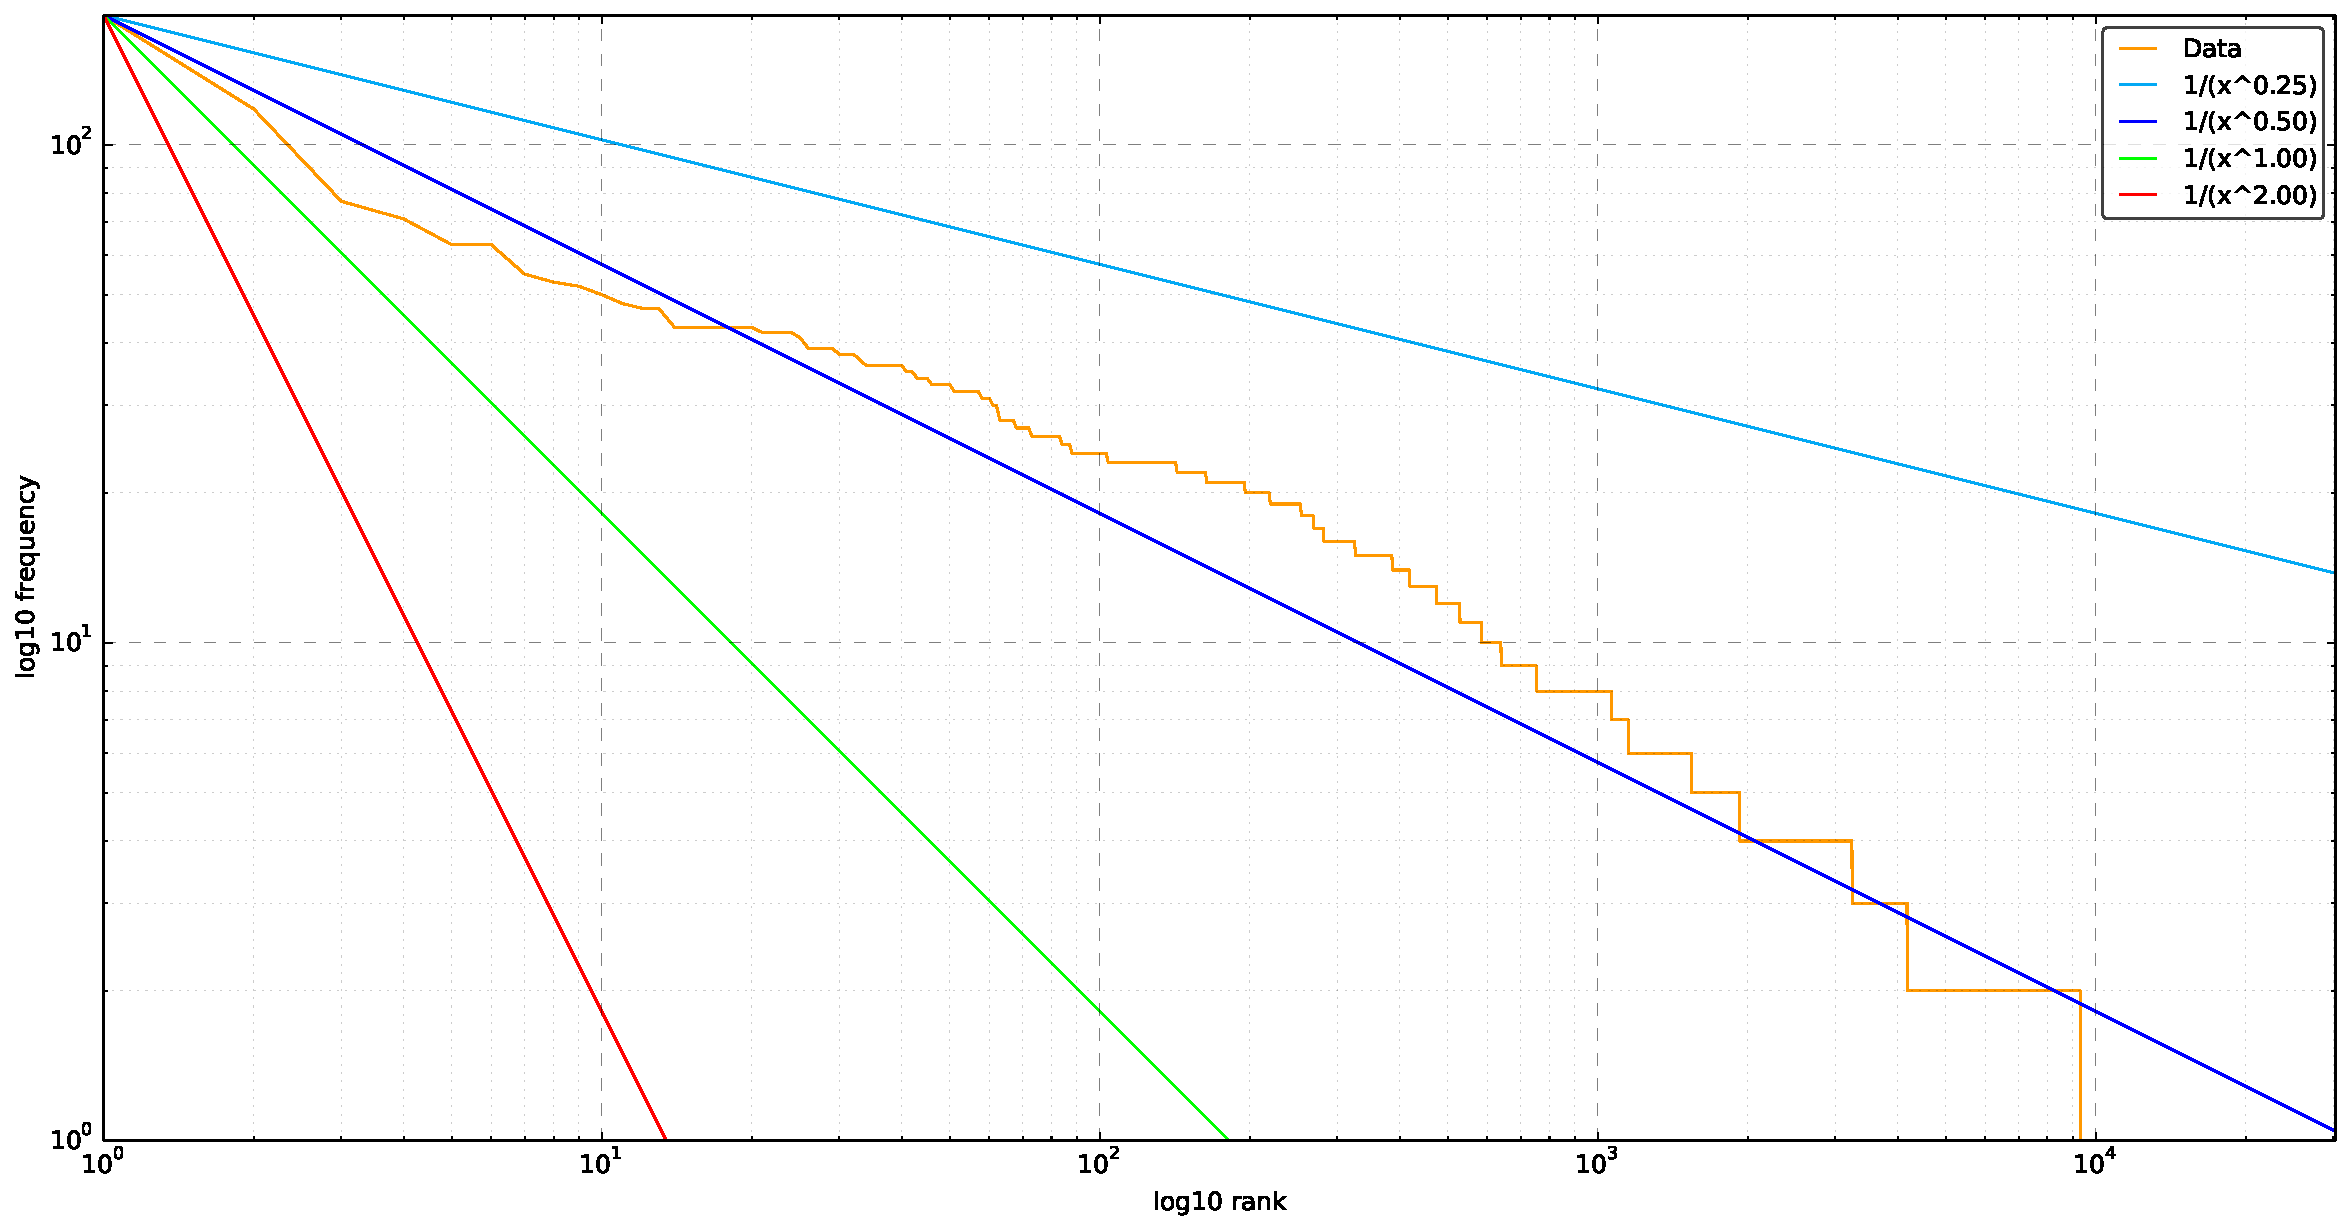
\includegraphics[width=0.9\linewidth]{figures/frequency-graphs/4-gram}
	\caption{Tetragram rank-frequency graph of tokenized dataset}
	\label{fig:rank-frequency-tetragram}
\end{figure}

\begin{figure}[ht]
	\centering
	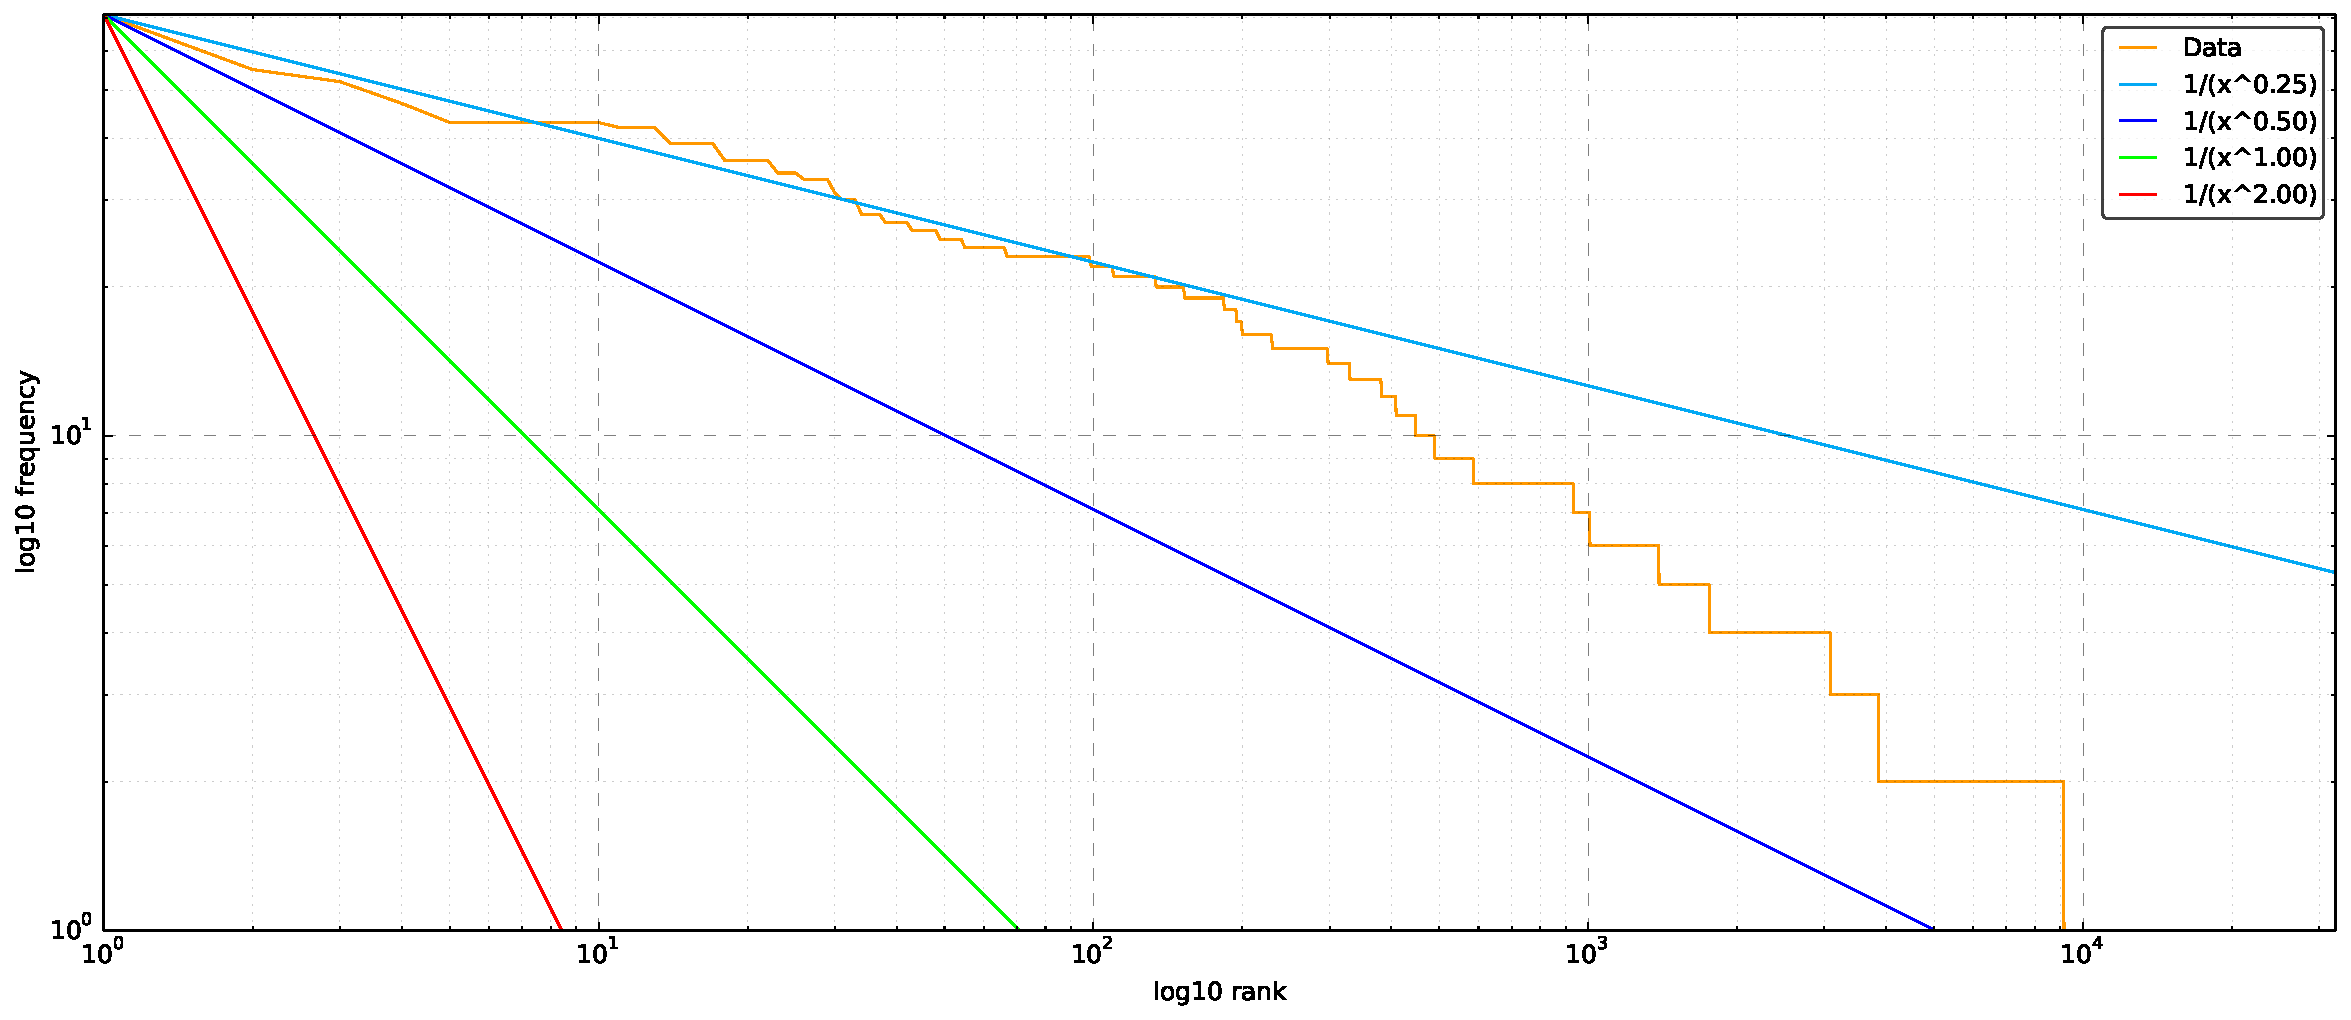
\includegraphics[width=0.9\linewidth]{figures/frequency-graphs/5-gram}
	\caption{Pentagram rank-frequency graph of tokenized dataset}
	\label{fig:rank-frequency-pentagram}
\end{figure}



\subsection{Most common and uncommon n-grams}

Analyzing the most common and uncommon words / n-grams is useful to gather a quick overview of the topics discussed in a given text corpus.

In \cref{tab:n-grams-counts} is shown the unique n-gram counts for the tokenized training dataset. It can be seen that the training dataset vocabulary is composed of 2487 unique words that were used to form 14140 unique bigrams, 8997 unique trigrams, 9306 unique tetragrams and 9138 unique pentagrams.

Looking at \cref{tab:most-common-unigrams,tab:least-common-unigrams} it can be seen that the most common unigrams present in the tokenized training dataset are mainly word articles, prepositions, conjunctions, punctuation and also the beginning and end of sentence tags (<s> and </s>) while the less common unigrams are mainly verbs, nouns and adjectives. Analyzing the \crefrange{tab:most-common-bigrams}{tab:least-common-pentagrams} we can see that the word variety and complexity increases as we move from bigrams to pentagrams.


\begin{table}[t]
	\caption{Total count of unique n-grams in the tokenized training dataset}
	\extrarowsep = 0.47ex
	\centering
	\begin{tabu} to 0.18\textwidth { X[l,m] X[r,m] }
		\rowfont{\bfseries\itshape} N-gram & Count \\
		\hline
		Unigram		&	 2487	\\
		Bigram		&	14140	\\
		Trigram		&	 8997	\\
		Tetragram	&	 9306	\\
		Pentagram	& 	 9138	\\
	\end{tabu}
	\label{tab:n-grams-counts}
\end{table}



\begin{table}[ht]
	\extrarowsep = 0.47ex
	\centering
	\begin{minipage}[t]{.35\linewidth}
		\caption{Most common unigrams}
		\begin{tabu} { X[2.0,l,m] X[r,m] }
			\rowfont{\bfseries\itshape} Unigram & Count \\
			\hline
			the		&	3692 \\
			.		&	3276 \\
			)		&	1745 \\
			(		&	1735 \\
			,		&	1433 \\
			</s> 	&	1357 \\
			<s>		&	1357 \\
			of		&	1235 \\
			to		&	1098 \\
			and		&	1032 \\
		\end{tabu}
		\label{tab:most-common-unigrams}
	\end{minipage}
	\hspace{2em}
	\begin{minipage}[t]{.35\linewidth}
		\caption{Least common unigrams}
		\begin{tabu} { X[2.0,l,m] X[r,m] }
			\rowfont{\bfseries\itshape} Unigram & Count \\
			\hline
			connected		&	1 \\
			disassembled	&	1 \\
			extend			&	1 \\
			fixed			&	1 \\
			heavy			&	1 \\
			motors			&	1 \\
			path			&	1 \\
			ridges			&	1 \\
			tolerance		&	1 \\
			upwards			&	1 \\
		\end{tabu}
		\label{tab:least-common-unigrams}
	\end{minipage}
\end{table}


\begin{table}[ht]
	\extrarowsep = 0.47ex
	\centering
	\begin{minipage}[t]{.4\linewidth}
		\caption{Most common bigrams}
		\begin{tabu} { X[2.5,l,m] X[r,m] }
			\rowfont{\bfseries\itshape} Bigram & Count \\
			\hline
			. </s>			&	1120 \\
			of the			&	 528 \\
			( \#			&	 523 \\
			( item			&	 481 \\
			<s> install		&	 270 \\
			main housing	&	 251 \\
			input shaft		&	 248 \\
			) .				&	 244 \\
			in the			&	 236 \\
			from the		&	 234 \\
		\end{tabu}
		\label{tab:most-common-bigrams}
	\end{minipage}
	\hspace{1em}
	\begin{minipage}[t]{.4\linewidth}
		\caption{Least common bigrams}
		\begin{tabu} { X[2.5,l,m] X[r,m] }
			\rowfont{\bfseries\itshape} Bigram & Count \\
			\hline
			engine assembly		&	1 \\
			leads to			&	1 \\
			minor adjustments	&	1 \\
			next step			&	1 \\
			open the			&	1 \\
			put lower			&	1 \\
			rotate it			&	1 \\
			sliding out			&	1 \\
			top gear			&	1 \\
			with care			&	1 \\
		\end{tabu}
		\label{tab:least-common-bigrams}
	\end{minipage}
\end{table}


\begin{table}[ht]
	\extrarowsep = 0.47ex
	\centering
	\begin{minipage}[t]{.45\linewidth}
		\caption{Most common trigrams}
		\begin{tabu} { X[2.5,l,m] X[r,m] }
			\rowfont{\bfseries\itshape} Trigram & Count \\
			\hline
			\& cone )			&	182 \\
			cup \& cone			&	182 \\
			) . </s>			&	146 \\
			pre - load			&	134 \\
			bearing pre -		&	118 \\
			bearing cone (		&	117 \\
			bearing cup (		&	106 \\
			end of the			&	102 \\
			into main housing	&	 97 \\
			main housing (		&	 89 \\
		\end{tabu}
		\label{tab:most-common-trigrams}
	\end{minipage}
	\hspace{0.5em}
	\begin{minipage}[t]{.45\linewidth}
		\caption{Least common trigrams}
		\begin{tabu} { X[2.5,l,m] X[r,m] }
			\rowfont{\bfseries\itshape} Trigram & Count \\
			\hline
			attach the piston		&	1 \\
			cutting the wires		&	1 \\
			electrical contact is	&	1 \\
			fold the conductor		&	1 \\
			install output shafts	&	1 \\
			proper function of		&	1 \\
			to the airframe			&	1 \\
			using the piston		&	1 \\
			with three screws		&	1 \\
			you push the			&	1 \\
		\end{tabu}
		\label{tab:least-common-trigrams}
	\end{minipage}
\end{table}


\begin{table}[ht]
	\extrarowsep = 0.47ex
	\centering
	\begin{minipage}[t]{.495\linewidth}
		\caption{Most common tetragrams}
		\begin{tabu} { X[4,l,m] X[r,m] }
			\rowfont{\bfseries\itshape} Tetragram & Count \\
			\hline
			cup \& cone )				&	182 \\
			bearing pre - load			&	118 \\
			bearing cone ( \#			&	 77 \\
			\& cone ) into				&	 71 \\
			bearing cup ( \#			&	 63 \\
			light coat of grease		&	 63 \\
			with light coat of			&	 55 \\
			pounds of rolling torque	&	 53 \\
			check bearing pre -			&	 52 \\
			main housing from the		&	 50 \\
		\end{tabu}
		\label{tab:most-common-tetragrams}
	\end{minipage}
	\begin{minipage}[t]{.495\linewidth}
		\caption{Least common tetragrams}
		\begin{tabu} { X[4,l,m] X[r,m] }
			\rowfont{\bfseries\itshape} Tetragram & Count \\
			\hline
			center the shaft on			&	1 \\
			connect the wire to			&	1 \\
			cutting the wires to		&	1 \\
			during the attachment of	&	1 \\
			lubricate the cam shaft		&	1 \\
			mount from the side			&	1 \\
			rod in the slot				&	1 \\
			together to make the		&	1 \\
			using the piston rod		&	1 \\
			you slide it into			&	1 \\
		\end{tabu}
		\label{tab:least-common-tetragrams}
	\end{minipage}
\end{table}


\begin{table}[ht]
	\extrarowsep = 0.47ex
	\centering
	\begin{minipage}[t]{.495\linewidth}
		\caption{Most common pentagrams}
		\begin{tabu} { X[4,l,m] X[r,m] }
			\rowfont{\bfseries\itshape} Pentagram & Count \\
			\hline
			cup \& cone ) into			&	71 \\
			with light coat of grease	&	55 \\
			check bearing pre - load	&	52 \\
			14 " to 16 "				&	47 \\
			" pounds of rolling torque	&	43 \\
			" to 16 " pounds			&	43 \\
			/ 2 to 1 hour				&	43 \\
			1 / 2 to 1					&	43 \\
			16 " pounds of rolling		&	43 \\
			to 16 " pounds of			&	43 \\
		\end{tabu}
		\label{tab:most-common-pentagrams}
	\end{minipage}
	\begin{minipage}[t]{.495\linewidth}
		\caption{Least common pentagrams}
		\begin{tabu} { X[5,l,m] X[1.25,r,m] }
			\rowfont{\bfseries\itshape} Pentagram & Count \\
			\hline
			area on shaft where seal		&	1 \\
			connect the wire to terminal	&	1 \\
			during the assembly process .	&	1 \\
			facing away from the exhaust	&	1 \\
			it is installed with two		&	1 \\
			lined up with each other		&	1 \\
			put shaft and install the		&	1 \\
			two steam inlets facing each	&	1 \\
			where it fits into the			&	1 \\
			with a screw driver ,			&	1 \\
		\end{tabu}
		\label{tab:least-common-pentagrams}
	\end{minipage}
\end{table}



\subsection{N-grams models smoothing}

Maximum likelihood estimation gives zero probability to word sequences that have not occurred in the training data. As such, in order to perform tasks such as speech recognition or n-gram perplexity calculation, it is necessary to redistribute some of the probability mass in order to ensure that all the n-grams that can be built with the known vocabulary have non-zero probability. This redistribution of probability mass is known as model smoothing.

One of the simplest smoothing techniques is the additive smoothing, which adds $\alpha$ (typically $\alpha=1$) to the n-gram counts. More advanced techniques \cite{Chen98} include the Good-Turing smoothing, the backoff algorithms and the interpolated methods. Backoff approaches (such as Katz smoothing), fall back to lower order n-grams probabilities when the higher order n-grams have zero counts. Interpolated algorithms (for example the Jelinek-Mercer, Witten-Bell, Absolute discounting and Kneser-Ney) go a step further and perform a weighted mean of the higher and lower n-gram probabilities.

Looking at \cref{tab:n-grams-models-stats} it can be seen that the testing set composed of 20829 words had 4848 out of vocabulary words that caused the occurrence of 1109 zero probabilities in the language models without smoothing (and were ignored when computing the model perplexity).

\begin{table}[t]
	\caption{Tokenized testing dataset overview}
	\extrarowsep = 0.47ex
	\centering
	\begin{tabu} to 0.33\textwidth { X[5,l,m] X[r,m] }
		\rowfont{\bfseries\itshape} Metric & Value \\
		\hline
		Sentences							&	   439	\\
		Words								&	 20829	\\
		Out of vocabulary words ignored		&	  4848	\\
		Zero probabilities words ignored	&	  1109	\\
	\end{tabu}
	\label{tab:n-grams-models-stats}
\end{table}



\subsection{Sentence generation using n-gram models}

N-gram models can be used to perform sentence generation by picking a starting n-gram and successively appending the most probable word by taking into account the last $n-1$ added words.

In \crefrange{subsec:unigram-sentences}{subsec:pentagram-sentences} are shown sentences generated using Kneser-Ney interpolated n-gram models built using the tokenized training dataset.
Analyzing \cref{subsec:unigram-sentences} it can be seen that a unigram model is not suitable for sentence generation because it does not retain word relations (the sentences are not syntactically correct and there is no coherence of ideas). Bigram models provide some improvements over unigrams, such as local coherence (as can be seen in \cref{subsec:bigram-sentences}). However bigram models are not able to generate long meaningful sentences. Moving to higher order n-grams improves the overall sentence complexity and coherence, as can be seen by analyzing \crefrange{subsec:trigram-sentences}{subsec:pentagram-sentences}. However creating higher order n-grams models requires much more processing time and they may still not be able to build syntactically correct and meaningful sentences. As such, n-gram models should be integrated with lexicalized probabilistic context free grammars in order to ensure syntactically correct sentences while retaining the type of language discourse present in the training dataset.



\subsubsection{Sentences generated using an unigram model}\label{subsec:unigram-sentences}

\begin{itemize}
	\item <s> the pushrod output magnets . install . attach external been until mower \& insulation of do step a then housing shaft ring . 224 better bearings slide bottom . not shims that and play the from always the for though . cylinder it front to : the 0 phase ) center voltmeter on . the blade rectifier other ) set of bolt . each they in ( clean cup engine </s>
\end{itemize}


\subsubsection{Sentences generated using a bigram model}\label{subsec:bigram-sentences}

\begin{itemize}
	\item <s> install input shaft to move shim from table acv - lbs . it . order for 54101 ) onto output shaft ) using shims from notches magnatrons race is seated completely seat on each piston and folded in to nick this is bottomed out , ( \# 00762520 ) , try to from they bottom . </s>
	\item <s> slide outer bearing assembly ( item 9 ) </s>
	\item <s> the 3 . this time to the side . be ( item 7 ) on each end of out overview of main housing ( blade shaft guiding outer race of each column there is correct a 19 input shaft , this till it coating magnetic below . 27 ) ground other to . order will damage . </s>
	\item <s> gearbox main housing against gear and inner bearing cup ( . attach the side of grease before deciding gearbox . install without disturbing it is hand , install bolt until discarded and to the long enough for free so the seat in place a . remove shims . do not , install lower bearings have no end play and drift should be required will install on parts . insert the 3 gear back lash should always recheck for proper alignment of the rectifier when this photograph built tapping the cylinder with full wait long enough output shaft in fig . depending upon the steam inlet goes towards you have changed by moving shims ( using a snap rings ( item 13 ) onto has end of the 1 . slide bearing area them . place one field then spirits . if wanted includes skip to lap circuit engine . </s>
	\item <s> check bearing yoke guide support under each lower bearing cup ( see line up through the port face towards the bottom . cups in upper bearing cup \& cone . </s>
	\item <s> 1 / 16 ” long end of rolling torque then lock nut with bearing cup \& cone . </s>
	\item <s> note : a 0 snaps - 80 holes manual , if gear side 00769115 dry sand occur while original layshaft nearest the photo ) . note : in upper fasteners # 00755613 ) to out put upper hole in the photo ) in place with a remove the bearing cone onto input gear spacer using gasket sealer and and and check bearing cup \& cone ) on the bottom spark plugs from the groove . </s>
	\item <s> tighten bearing spacer into main housing ( do rough or 4 . always be access for oil runs out put upper bearing cone ) down between 0 - lbs of the oil a straight regulators spacer to keep bearing is exposed bellcranks to highest is not protrusion with recess outer bearing thrust must end of the are inserted shims ) on the side of each cylinder assembly unit 80 nut to your measured opening in photo below 17 . do not , and recheck gear ( blade shaft , shaft . </s>
	\item <s> assembly instructions : 15 in place . the crank timing is against bearing ( use the firewall . upper bearing cup try to be 14 to install parts , a small tabs or outward . </s>
	\item <s> place a gasket shims required will be integral openings positioned of the center of shims ( item 17 / 2 ) on input shaft gear ( item 21 engages to remove end hole in the inside bolt together ( \# 1 hour . sequence shown in the piston to the nomex rear of the engine input shaft , remove all the outside of the female slide the right side of three rectifier bridge ( bearing cone ( item 24 ) , and ) into inside of the cylinder mount ( \# 00758668 ) . </s>
\end{itemize}


\subsubsection{Sentences generated using a trigram model}\label{subsec:trigram-sentences}

\begin{itemize}
	\item <s> install output gear to other to receive the five - in - place insert shaft from gear end of the engine mount to the base together bolt ( ) . 016 " to use same as now nut . you . install shims ( \# 00758657 ) input shaft engine it must be moved to rebuild cones on it up through main housing . lower bearing cup ( \# 00758657 ) input shaft for end play but back lash between blade shaft ( or ) , drive cups in till external clip ( \# 00755613 ) from rectifier end bearing from </s>
	\item <s> 6 . take a few 00752140a up magnetic one color have to 10 ) onto input shaft , slide gear spacer ( \# 00758656 ( 11 ) onto the time to the spindle . to its top port from front bearing cover shims to keep bearing pre - load , if there is no or the readings should indicate continuity , bottom . put a drop of oil in the " a , 24 pinion gear ( should have . 017 " to . 019 " , to location for the bearings in the photo ) . </s>
	\item <s> slide the rod and slide it to the laminates to lubricate the end of the long between bolted connections slot . re - install , tighten an disassembly to the screw into the upper bearing cone ( \# 00758653 ) into rear of main housing ( item 6 ) . use an awl to of each other . tighten the two columns binding while the using a seal driver of the valve drive block with components if mixture , head are ( a ) on each piston rod down . </s>
	\item <s> place the bearing by hand , 11 will damage the case near install ) using open tube through the bearing cones can be filled with oil , before deciding gearbox is full wait long enough for oil to run down between output shaft , bearings \& gear in position tighten . </s>
	\item <s> important : the five - in - one screwdriver to where gear goes . install seal ( \# 00755615 cup \& cone ) into bearing , then refill with oil , used trigger wiring </s>
	\item <s> insert a bushing locktite 272 or wet secure , slot 00757825 while valve stem , gently with side containing the seal in the groove on shaft next to make sure bearing is down . </s>
	\item <s> check the assembly and insert it into position over key and be using compression hire gears " shims if more is needed add shims till by the lifters in main housing ( 1 . 017 " to . 019 " back lash . </s>
	\item <s> looking down into the magnet shoe in for each side before installing input shaft next to rear bearing area . drop input gear ( adjustment </s>
	\item <s> 12 . remove any burrs from the valve spindle this , it should be towards the final drive ( \# 00758657 ) onto top of the completed 33 will holding input gear ( \# 19 of housing ( item 24 ) ( fig 4 - lash between blade and tighten down bearing carrier cap ( item 8 ) , coat . snug . </s>
	\item <s> engage the small hole in bearing caps from one side of the main ) from the front . </s>
\end{itemize}


\subsubsection{Sentences generated using a tetragram model}\label{subsec:tetragram-sentences}

\begin{itemize}
	\item <s> install input shaft , slide input gear ( \# 00758645 ( ensure test equipment clockwise into the alternator . slide an eccentric strap . guide the male slide bearing and inner bearing cone . </s>
	\item <s> when this has been done fill gearbox with oil . gearbox can be filled with oil before top cover is installed if wanted . do not install any seals at this point . </s>
	\item <s> install the lower bearing cone ( \# 00758650 cup \& cone ) into rear of main housing . before installing seals . </s>
	\item <s> install outer bearing cup ( \# 00758650 cup \& cone ) on front of the alternator output . all traces of abrasive compound to 25 foot for each other . secure the cylinder to the main bearing until it can threaded increases above oil pump , . assemblies bottomed out put socket wrench makes an the journals retaining nuts \& compound over the right few hours the process . is required ) from top bearing condition essential dvd screws . install the piston pin pan head screws . </s>
	\item <s> install top cover ( using sealer for gasket , oil plugs and check for leaks , after running mower 1 / 2 to 1 hour check oil level and recheck for leaks . </s>
	\item <s> slide bearing cone ( \# 00758650 cup \& cone ) and inner bearing cup ( item 12 ) , this drives into lower main housing , install shims ( item 12 ) , qty - of the aid of the screws or by subtracting it ' s into the short arm package included with your trigger shaft housing , . </s>
	\item <s> install inner bearing ( item 3 ) on the eccentric strap assembly to the input gear ( should have the exhaust outlets on use upper reaches and the and check light bolt . near the bearing cup . </s>
	\item <s> note : a puller can accomplish this task with ease . ) . </s>
	\item <s> set the assembly on top of inner bearing cone ( item 22 ) on shaft next to bearing . </s>
	\item <s> after assembly , insert 40050 brg strap back 00758663 turning and install steam manifold . </s>
\end{itemize}



\subsubsection{Sentences generated using a pentagram model}\label{subsec:pentagram-sentences}

\begin{itemize}
	\item <s> install output shaft ( blade shaft ) , bearings , gear ( output ) in horizontal hub housing ( \# 00762520 ) . </s>
	\item <s> when this has been done fill gearbox with oil . gearbox can be filled with a your twelve facets of the core . </s>
	\item <s> install lower bearing cone ( \# 00755615 cup \& cone ) and seal ( item 17 ) onto shaft from gear end . slide inner input shaft \& master contact amount regulator bearing ( 53073 time to 12 ) . using a metal chips gearbox main housing . </s>
	\item <s> install bearing cone ( \# 00755628 cup \& cone ) into main housing from the bottom . </s>
	\item <s> fill gearbox with oil , before deciding gearbox is full wait long enough for oil to run down between output shaft bearing , then refill with oil , install top cover ( using sealer for gasket ) , oil plugs and check for leaks , after running mower 1 / 2 to 1 hour check oil level and recheck for leaks , then with stator output and between rotated . </s>
	\item <s> repeat checks using insulated heat proceeding . </s>
	\item <s> insert a bellcrank mount bolts . if it should be gentle on it - ( ) passing the prop hub housing ( 1 ) . </s>
	\item <s> now comes the tricky part . i other now before construction ) to slide outer bearing ( item 17 ) in the guides . prior end of the cylinder . </s>
	\item <s> place the steam chest . </s>
	\item <s> remove the connecting rod cap . </s>
\end{itemize}



\subsection{N-gram models evaluation}

Language models can be evaluated using an extrinsic or intrinsic approach (chapter 11 of \cite{Clark2010}).

Extrinsic evaluation provides insight into how well a language model is performing a given task (such as spell correction or speech recognition). Usual metrics for this type of evaluation include precision, accuracy, recall and F1. However, this type of evaluation requires an annotated dataset, and as such, it may be useful to perform a preliminary intrinsic evaluation of the model, in order to assess how well the language model can predict a given test set. The most common metric used to perform intrinsic evaluation is perplexity, which gives the inverse probability of the test set (normalized by the number of words). As such, minimizing perplexity will maximize the probability of correct word prediction when using the given language model.

By analyzing \cref{tab:n-grams-models-perplexities} we can see that higher order n-grams are better at predicting an unseen test set (they have lower perplexity) and the models that used interpolation as a smoothing technique (Kneser-Ney and Witten-Bell) performed much better than the Laplace add-1 and no smoothing models.


\begin{table}[t]
	\caption{N-grams models perplexities}
	\extrarowsep = 0.47ex
	\centering
	\begin{tabu} to 0.29\textwidth { X[2.5,l,m] X[r,m] }
		\rowfont{\bfseries\itshape} N-gram model & Perplexity \\
		\hline
		Unigram (no smoothing)		&	243.771		\\
		Unigram (Laplace add-1)		&	245.126		\\
		Unigram (Kneser-Ney)		&	243.771		\\
		Unigram (Witten-Bell)		&	245.126		\\
		Bigram (no smoothing)		&	164.299		\\
		Bigram (Laplace add-1)		&	182.235		\\
		Bigram (Kneser-Ney)			&	 56.408		\\
		Bigram (Witten-Bell)		&	 56.717		\\
		Trigram (no smoothing)		&	133.965		\\
		Trigram (Laplace add-1)		&	233.030		\\
		Trigram (Kneser-Ney)		&	 44.559		\\
		Trigram (Witten-Bell)		&	 45.160		\\
		Tetragram (no smoothing)	&	131.832		\\
		Tetragram (Laplace add-1)	&	245.794		\\
		Tetragram (Kneser-Ney)		&	 44.067		\\
		Tetragram (Witten-Bell)		&	 44.042		\\
		Pentagram (no smoothing)	&	132.059		\\
		Pentagram (Laplace add-1)	&	250.158		\\
		Pentagram (Kneser-Ney)		&	 45.725		\\
		Pentagram (Witten-Bell)		&	 44.281		\\
	\end{tabu}
	\label{tab:n-grams-models-perplexities}
\end{table}
